%!TEX root=../tax-democracy-held.tex
%don't write condescendingly about voters.

%or maybe, call this tax and democracy?

\begin{quote}
	\emph{``Politics is like the fabled Sphinx:
	It devours all those who cannot solve its riddles.''}
	\\*
	--- Antoine de Rivarol
\end{quote}

\begin{quote}
	\emph{``A popular government, without popular information or the means of acquiring it, is but a prologue to a farce or a tragedy, or perhaps both.''}
	\\*
	--- James Madison (1822):\ Letter to W.T.~Barry
\end{quote}

\begin{quote}
	\emph{``All of these reforms cannot occur unless people learn to think about taxes without the isolation effect we have found.
	They need to see the big picture.''}
	\\*
	--- Edward J.~\citet[23]{McCaffery2003}
\end{quote}

%CIT works with  concentrated interested because small firms suffer from ti, big ones can calculate themselves to zero

%Deliberation is more than a method, here.
%Tax is more than a case, here

%this is all Olaf:
%consider, says Olaf, Habermas (Theory of communicative action) on "fragmentisierung des Alltagswissen) /  assumed theoretical link:
%if you want to hide injustice, than you'd best do it in a really complex system, like tax.
%/ this can be answered best by comparing tax to other topical areas, where people's knowledge is less biased, and where injustice is not a concern // Olaf says:
%knowledge is key.


%Farrar
        %* (334) 3 hypothesis
%      * attitudes (=continuous dispositions towards policy alternatives) change (individua/gross and aggregate/net)
   %   * preferences (ordinal rankings of alternatives) become closer to single-peakedness (no cyclical majorities of the sort identified by Condorcet and Arrow)
%      * both effects are stronger (interaction!) for less salient issues (tax? vs.\ Stuttgart 21)
%   * 335:
%the driving effect is learning.
%the people who learn the most change the most and are the most single-peaked
%   * now this article tests salience vs.\ deliberation (people are randomly assigned to 2 issues, salient/non-salient)
%   * single-peakedness means there is a Condorcet winner (an alternative that beats, or is tied with, all others in pairwise majority voting)
%   * people may become more single-peaked for different reasons:
%      * adopt what (elites) other people think
%      * acquire a more shared, intersubjective understanding
%      * indepedently excogitate a natural ordering compelled by logic
%   * i'm not happy about the scope of the deliberation; they seemed very micro, very confined.
%I would think that my setting (a mixed economy) is a lot broader and requires a lot less axioms.

%for an example of empirical work on deliberation, cite Farrar et al 2003:
%single-peakedness and structuration increases after deliberation.
%Tax is exactly the example that this, in a pluralist debate, is not the case.

%n some way, the fact that pluralism no longer works (because of positive sum situations) should not surprise us:
%that is the story of societal development over all.
%It is actually good news, too:
%We don't want a zero-sum society, that is dangerous.

%Maybe, in the past, things were a little more zero-sum, and we should be grateful that they no longer are.
%But more importantly, in the past, as societal differentiation was at a lower level, issues were probably not as complicated and interests less finely concentrated (the sugar subsidy thing).
%Or maybe not.

%random note
	%there are constraints in policy.
%That is the difference between ideology and feasible and deisrable hypotheticals.
%But you have to break it down further:
%it is doable, in that it is MATERIALLY possible, without violence, or otherwise restraining liberal freedoms (and democracy, too).
%So, if you come to the conclusion, this tax won't work, it'll cost too much evasion, the only alternative would be widespread violence, then it's not doable, we'll have to find an icnremental way into the future, even though in that scenario, you should be clear about the ultimate ends, the finality of progress.
%Just the route that you take will have to be a littler longer and windy.
%There is however one thing that you absolutely cannot consider for diablity:
%and that is:
%"can I sell it to the people".
%That is not enlightenment; that is not democracy, anything that can be done materially, must be explainable.
%Cororally:
%understandings aren't pre-social, or preferences.
%If you assume that preferences are pre-social, it becomes a merely empirical question of whether a positive question of whether can or cannot be done.
%The only question that remains is in that scenario:
%is the aggregation mechanism working efficiently.
%And that's more or less the Lijphart debate, is it efficiency and equitably, and will depend largely on the equity norm you choosse:
%consensus vs.\ majoritarianism.
%If you allow for the fact that preferences are essentially social, or in a more malignely put, that there are unenlightened preferences, even false class consciousness, or in line with the deliberative fiew, that on an entological level, preferences CANNOT be pre-social )and there's an evolutionary argument to that, because property isn't presocial).
%If you think they are social and contingent, and that some of the preferences are non-preferences, then, you're coming into a world where you need to explain things and the only variable for that kind of discussion is a FIRST best criterion, the criterion of is this materially possible and desirable, but not:
%can i sell this.
%"Can I sell this" is the market metaphor, which assumes preferences to be given (also misleadingly thing advertisement).
%This might be another link:
%markets assume presocial preferences, and they err, eg.
%on expenditure cascades and other form of induced demand or relative spending.
%(essentially SOCIAL preferences!) and that is true in democracies, too.
%Again, put it clearly that my position is one of reform, never of revoltuoin.
%Don't ask for a new man, just ask for some new policy.
%Also point out, tidbit from economist (polar bear):
%don't do policy-based evidence making.

%I think the nature of Human beings IS Subjekt to empirical Investigation.
 	%So IS human cognition,
	%But, qua enlightenment what is NOT meaningful subject to empirical investigation is the process of political change be it welfare state or IR, only whether it dies what it's supposed to do.
	%This is far more than deliberative theory, it's deliberative social science.

\begin{figure}[htbp]
	\centering
	%
\includegraphics[width=1\textwidth]{asu-poster.jpg}
	%this guy has moved to g+ pics, not sure I still need that.
	\caption[Entrepreneurship Campaign Poster]{Campaign Poster by a Business Lobby, Berlin 2009}
	\begin{flushleft}
		\scriptsize{The poster reads:
			\begin{quote}
				\emph{``You can take away our money.
				Or you can let us spend it.''}
			\end{quote}
			The campaign is signed by \href{http://www.familienunternehmer.eu}{Die Familienunternehmer ASU e.V.} (family-owned business), formerly known as Arbeitsgemeinschaft Selbst\"{a}ndiger Unternehmer (working group of self-employed entrepreneurs).}
	\end{flushleft}
	\label{fig:asu-poster}
\end{figure}

%- complexity
%- uncertainty

%My misunderstandings of tax are like the linguists Sapir-worf hypothesis

\section{Misunderstandings}

Here, as well, I find conspicuous signs:
a public thoroughly confused about the abstractions and trade-offs of their economy and marred by dysfunctions of pluralist democracy.
These leads run deep, too, implicating the entire edifice.
To the questions of what democracy \hyperref[chap:desirable-democracy]{should} (\autoref{chap:desirable-democracy}) an On closer inspection, pluralism may be a minimal formulation of democracy, skeptical about what people can do and restrictive about what democracy should do.
Once a historical accomplishment, the institutions of representative democracy are today outmatched by the vast complexity, and tightly concentrated special interest of the modern economy and needlessly conservative about human nature.


\subsection[Bastard Keynesianism]{Bastard Keynesianism \\--- Arbitrarily High, Real Saving \emph{is} Possible}
%"Bastard-Keynesianismus":
%Der weit verbreitete (Irr)glaube, eine Volkswirtschaft könne nicht beliebig viel Sparen, weil dann die "Binnennachfrage" zusammenbricht.
%Dies ist falsch, da auch Investitionen, nicht nur Konsum, Nachfrage sind.
%Wenn die Volkswirtschaft langsam genug die Sparquote hochfährt, entsteht keine Nachfragekrise.
%Als Folge dieses Missverständnisses (so meine Hypothese) können viele Bürger systematisch über eine sparfreundliche Steuer nicht nachdenken.
%or known as:
%franckenstein keynesianismus,  is when we can have no arbitrary savings rate.

%addition to Frankenstein Keynesianism.
%Keynes is concerned about output, because of Keynes, we are concerned with GPD (even though he didnÄt like it).
%But GDP was never meant to be a sufficient condition (but merely necessary in the short and medium run) for prosperity.
%It measures only activity, not what we add to the stock of the economy.
%In part, as a result, by looking only at GDP, we get very confused about what kind of savings rates we can have.

%frankenstein hayekianism:
%Frankenstein Hayekianism is when we can have no arbitrary state rate.

%frankenstein beggar-thy-neighbor:
%when a lot of exports are good


\subsection[Technocratic Myopia]{Technocratic Myopia \\--- Greater, Real Saving \emph{is} Necessary}
%People think we save enough (real myopia) or, more specifically, they fall for nominal indicators.


\subsection[Government vs Market]{Government vs Market \\--- Societies \emph{can} Choose Arbitrary Government Quotas}
%state vs market is a zero/positive sum game, not ``mehr netto vom brutto''
\subsubsection{Zero-Sum}
	%trade-offs graph/coordinate space of the mixed economy

%	negative sum:
%People think government harms the economy (it does)

\subsubsection{Positive Sum}

\subsection{Cooperation Problem of Tax}
%congruence or arbitrage

\subsection{Confusion of Pigovian and Revenue/Redistributive Taxes}
%redistribution and revenue are one, others are different.
%show table.

\subsection{Only Natural Persons are Moral Subjects}
%you shouldn't tax corporations
%People want to tax non-natural persons (corporations as people)

\subsection[Flypaper Theory]{Flypaper Theory \\--- The Incidence of Taxation is \emph{not} Trivial}
%you can't tax corporations
%People think we can distribute the burden of taxation at will (flypaper theory 0-sum)

\subsection{Markets Will React with DWLs}

%"Flypaper Theory of Tax":
%Der weit verbreitete (Irr)glaube, der Gesetzgeber könne die Steuerlast qua fiat verteilen, also etwa durch die Besteuerung von Unternehmen.
%Tatsächlich ist die reale Inzidenz von Steuern komplexer (sie hängt von den relativen Preiselastizitäten der Marktteilnehmer ab).
%Als Folge dieses Missverständnisses (so meine Hypothese) überschätzen viele Bürger systematisch die Möglichkeit von indirekten, insbesondere Unternehmenssteuern.
%(so ähnlich haben dies auch McCaffery und Baron gezeigt, allerdings für indirekte Steuern im Allgemeinen).

 %  * flypaper theory of tax:
%taxing corporations is stupid.
%but it's also necessary.
%but people like it (ARlen and Weiss 1994, as cited in McCaffery Baron 2003:
%7)

\begin{landscape}
 \begin{figure}[htbp]
	\begin{center}
	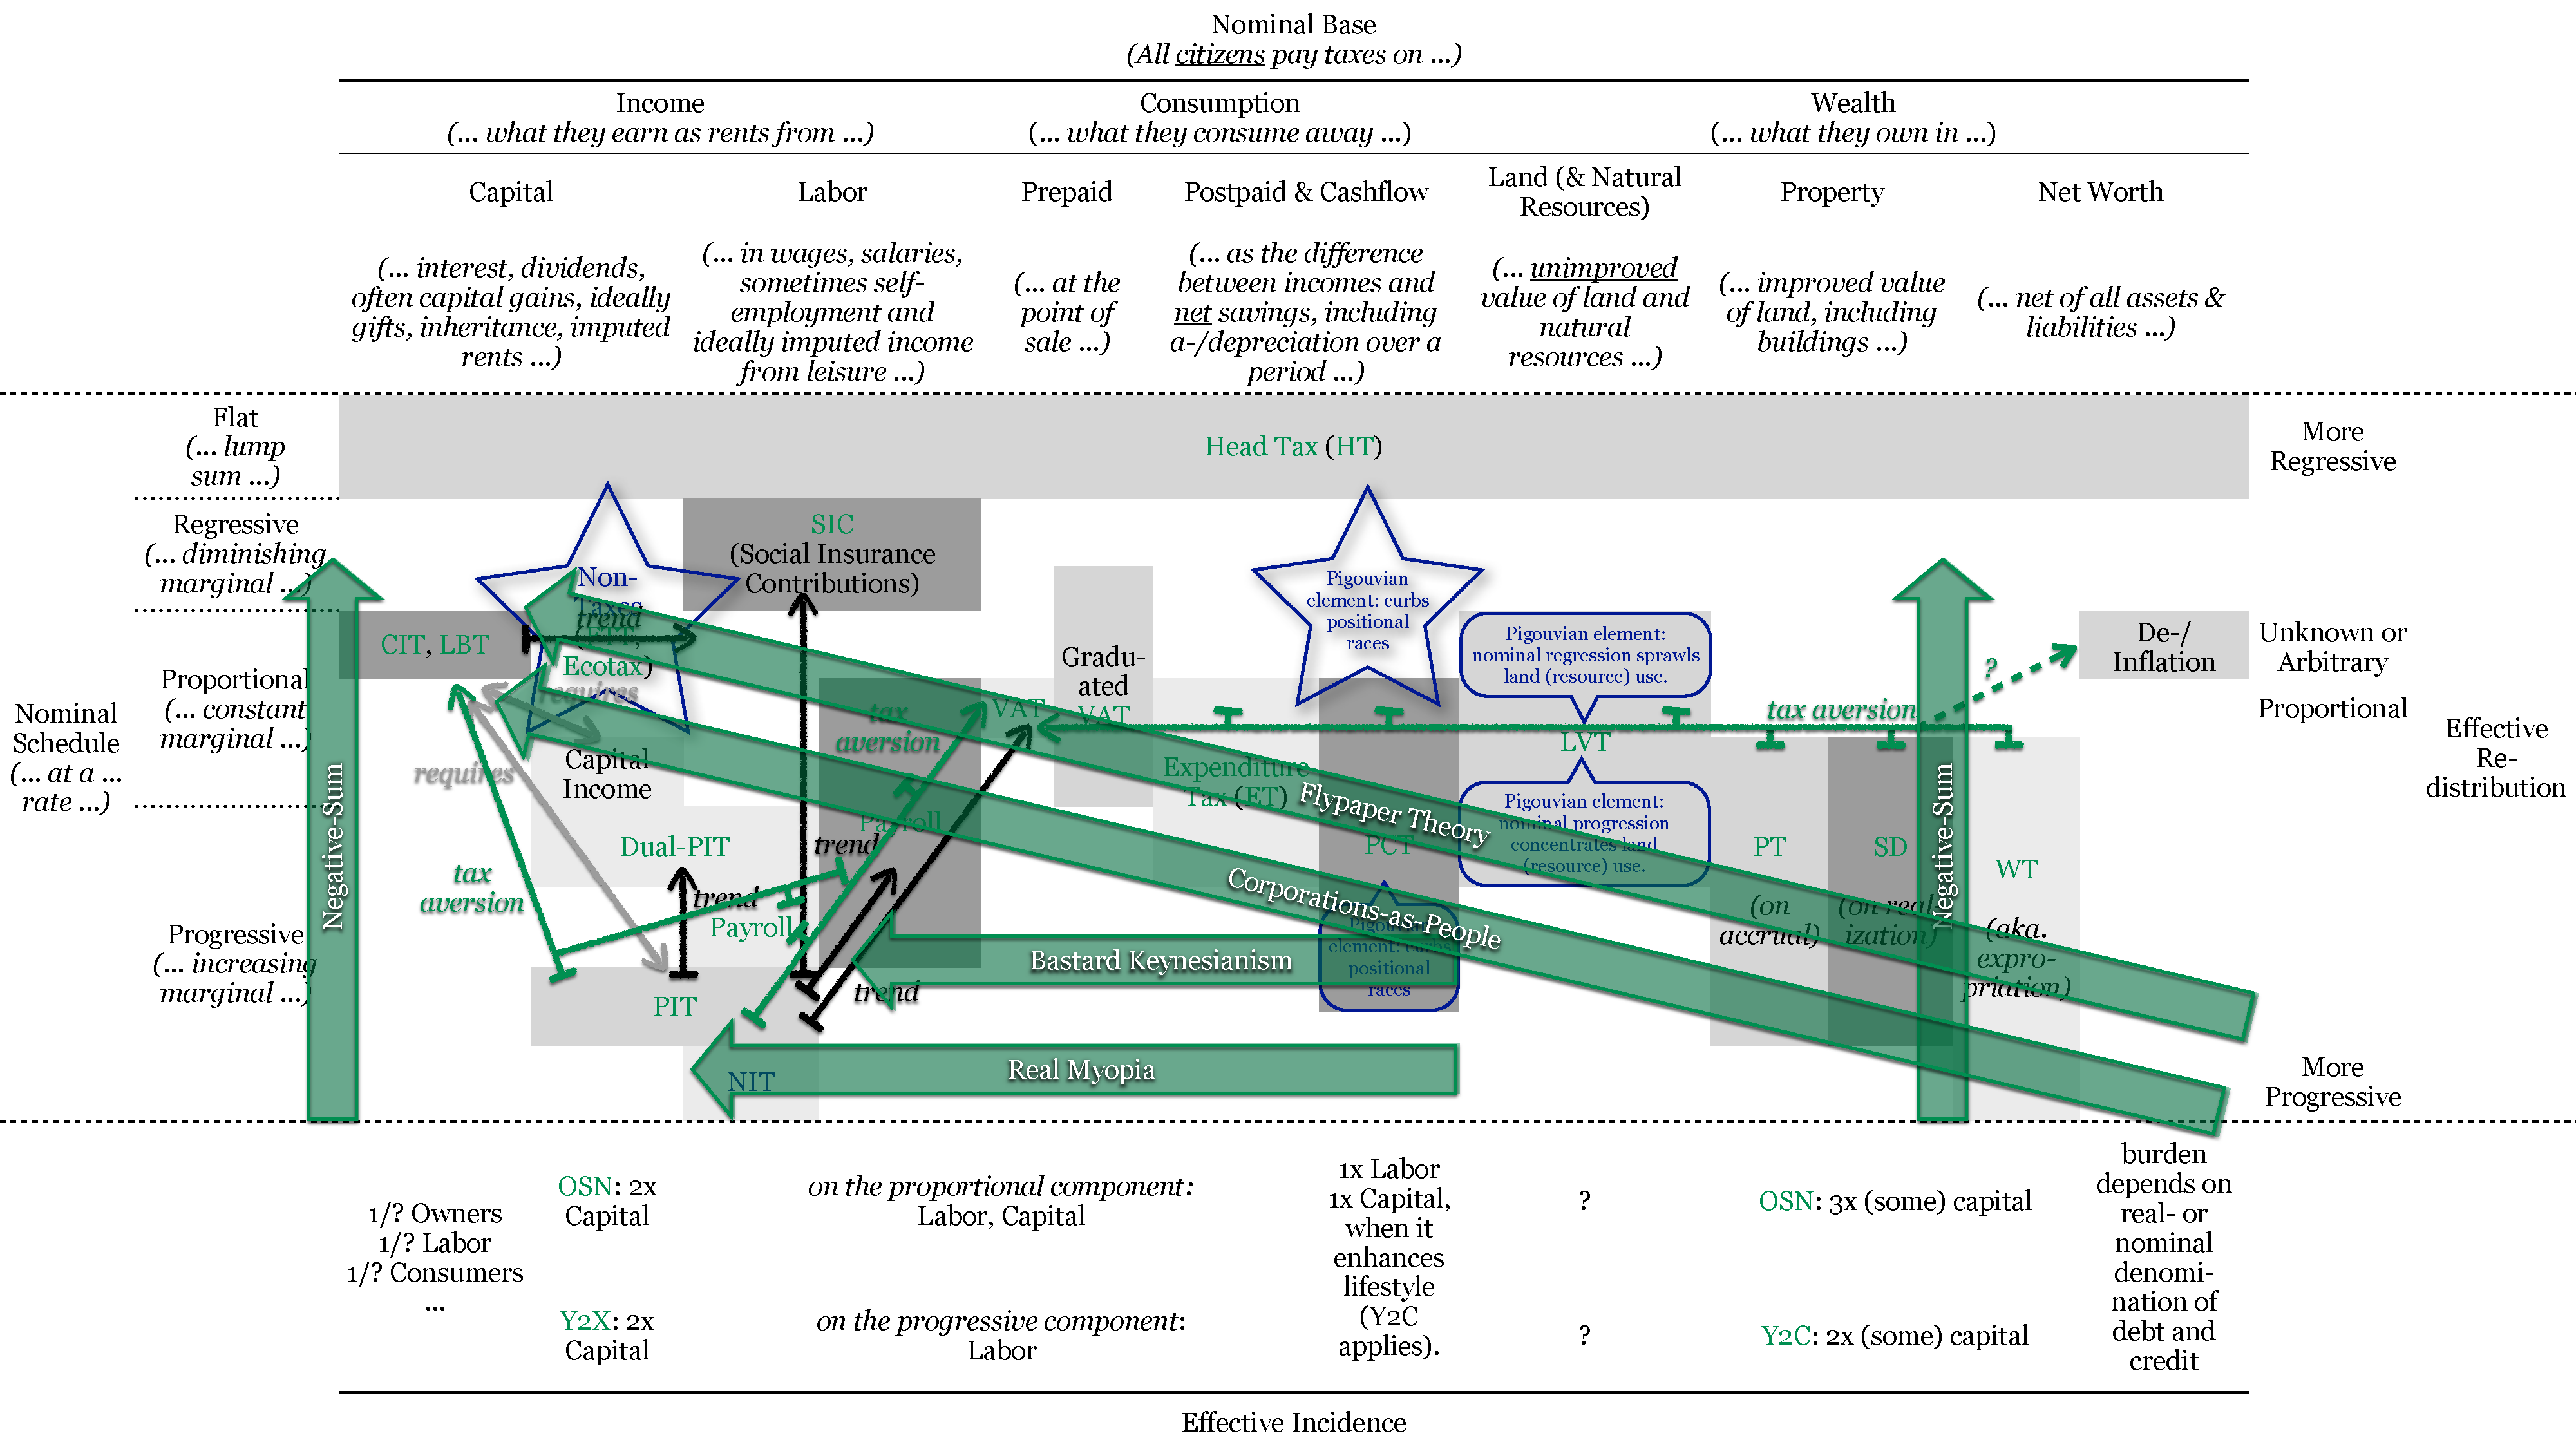
\includegraphics[width=1\linewidth]{tax-with-all}
	\caption[The Vector Field of Taxes with Systematic Biases]{The Vector Field of Taxes with Systematic Biases}
	\label{fig:tax-with-all}
	\end{center}
	%!TEX root=../tax-democracy-held.tex

\scriptsize{
	\glsfirst{CIT},
	\glsfirst{Dual-PIT},
	\glsfirst{Ecotax},
	\glsfirst{ET},
	\glsfirst{FTT},
	\glsfirst{LBT},
	\glsfirst{LVT},
	\glsfirst{NIT},
	\glsfirst{OSN},
	\glsfirst{PCT},
	\glsfirst{Payroll},
	\glsfirst{PT},
	\glsfirst{SD},
	\glsfirst{VAT},
	\glsfirst{WT},
	\glsfirst{Y2C} and

	\hyperref[sec:distributive-effects-of-inflation]{the distributive effects of in- and deflation} (p.~\pageref{sec:distributive-effects-of-inflation}).
}
\end{figure}
\end{landscape}

\subsection[False Omniscience]{False Omniscience \\--- Flows of Income \emph{Cannot} be Easily Known}

\subsection{Tax Aversion}
%this is (\cite{McCaffery2003}:
%12ff), people simply react to the labeling of ``tax'' even when the economics are the same as for a ``payment''.

%Tax aversion effect:
%people react (negatively) to the label "tax".
%People prefer indirect taxes (tax aversion effect)

\subsection{Metric Effect and Progressivity Illusion}
%this is (\cite{McCaffery2003}:
%15ff) people want more progressivity in percent than in dollar terms.

\subsection{Penalty Aversion and the Schelling Effect}
%this is (\cite{McCaffery2003}:
%17ff) people prefer bonuses to penalties, even when they are the same; people reverse their tax preferences according to the wording under the Schelling effect (together with some illusion of progressivity).
%Schelling effect:
%People prefer bonuses over penalties

\subsection{Disaggregation Bias}
%this is (\cite{McCaffery2003}:
%19ff) note that this relates to my point on ordoliberal hygiene; and wrapping different taxes in one tax.
%People don't understand that they can make up for the schedule of one tax with the schedule of the other tax (when the BASE is the same!) This is key!

%Disaggregation bias:
%People do not integrate different taxes on the same base

\begin{landscape}
 \begin{figure}[htbp]
	\begin{center}
	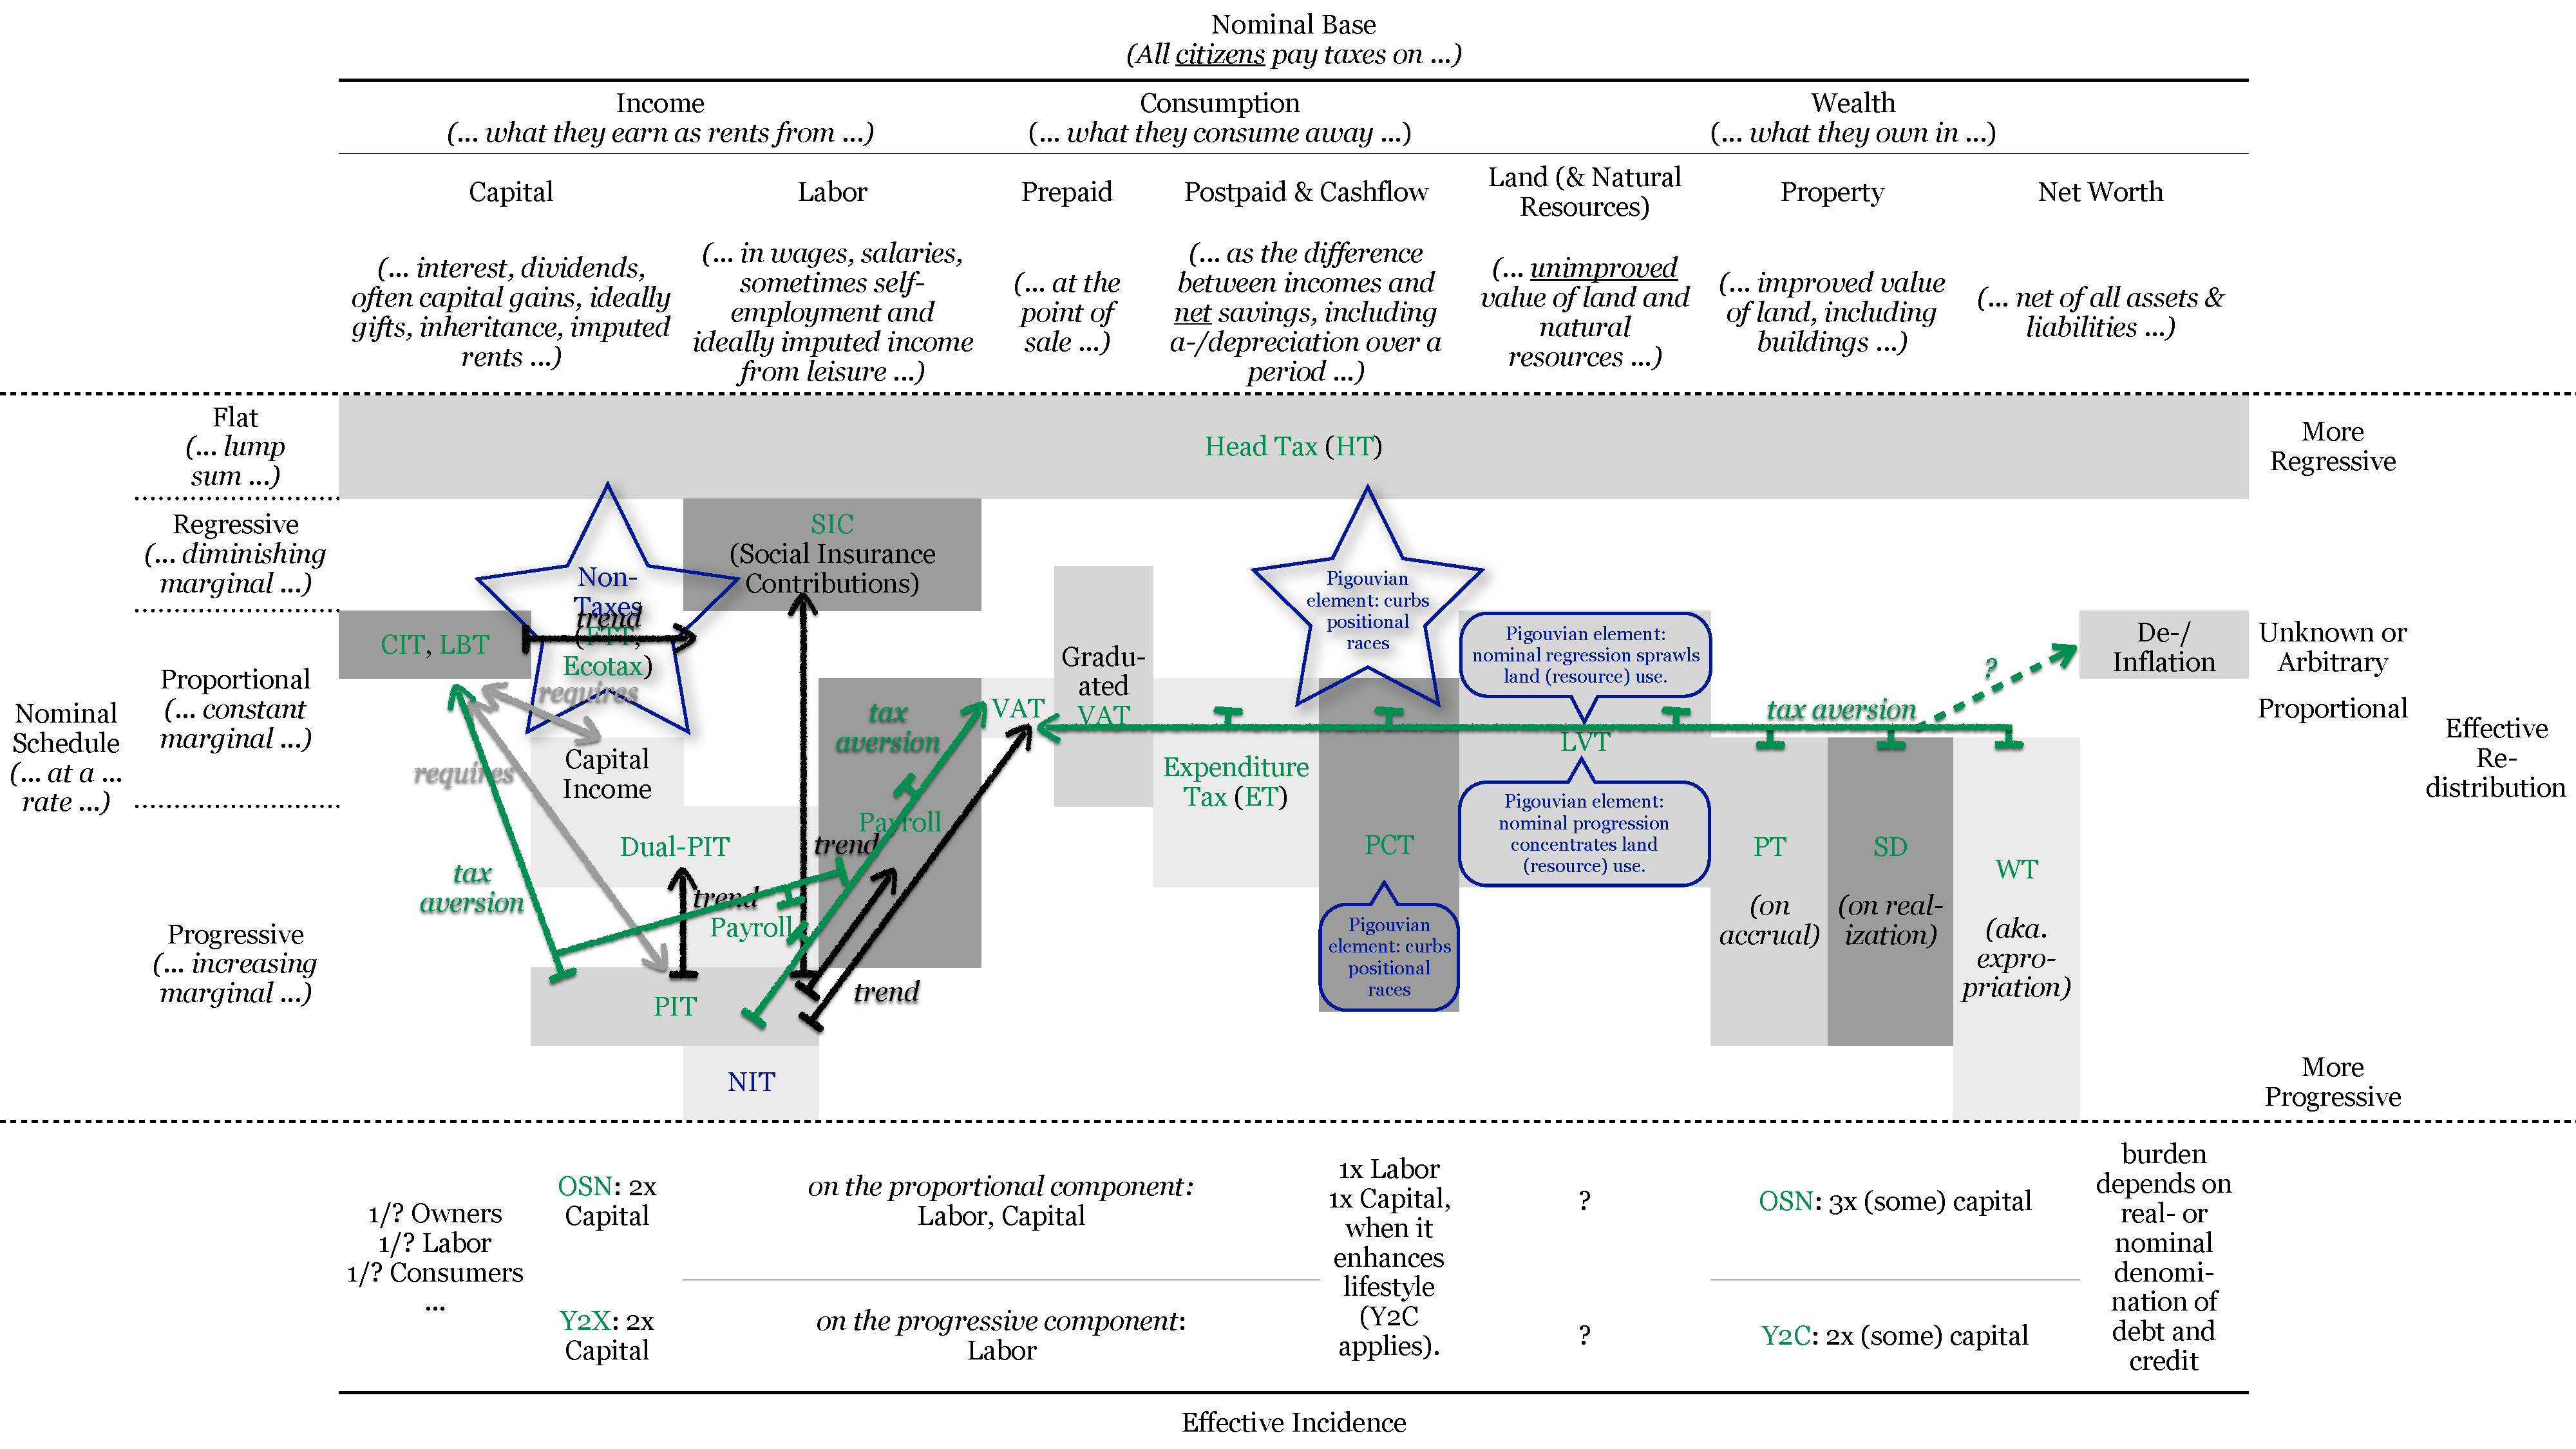
\includegraphics[width=1\linewidth]{tax-with-biases.pdf}
	\caption[The Vector Field of Taxes with Systematic Biases]{The Vector Field of Taxes with Systematic Biases}
	\label{fig:tax-with-biases}
	\end{center}
	%!TEX root=../tax-democracy-held.tex

\scriptsize{
	\glsfirst{CIT},
	\glsfirst{Dual-PIT},
	\glsfirst{Ecotax},
	\glsfirst{ET},
	\glsfirst{FTT},
	\glsfirst{LBT},
	\glsfirst{LVT},
	\glsfirst{NIT},
	\glsfirst{OSN},
	\glsfirst{PCT},
	\glsfirst{Payroll},
	\glsfirst{PT},
	\glsfirst{SD},
	\glsfirst{VAT},
	\glsfirst{WT},
	\glsfirst{Y2C} and

	\hyperref[sec:distributive-effects-of-inflation]{the distributive effects of in- and deflation} (p.~\pageref{sec:distributive-effects-of-inflation}).
}
\end{figure}
\end{landscape}

%consider ``small is beautiful'' by Schumacher.
%It's not about the size.
%Look for Brian sth.
%pictures of dead malls.
%Small is beautiful always implied that bastard keynesianism was wrong.
%Cite Bush "I encourage you to shop more".
%Here's a tax that does away with thos.

%McCaffery, E.
%J., & Baron, J.
%(2003).
%Heuristics and Biases in Thinking about Tax.
%Los Angeles, CA.
%doi:
%10.2139/ssrn.467440.

%   * 7:
%Our most general hypothesis is that we expected to find a wide range of heuristics and biases in people’s understanding of and attitudes about tax.
%The general complexity of the subject matter, the low benefits for any individual to obtain on a personal level from fully understanding it, the absence of any general, widely available mechanism to debias or educate people about tax, can all be expected to, if anything, make the usual heuristics and biases more acute in the field of tax.
%people's results differ if they call it "tax" vs.\ "payment" metric effect (people want less progression in dollar terms than in % terms(they don't understand the difference b/w payroll and income tax,bottom line:
%hidden taxes will flourish (22)

%drawing on Simon (1955), Kahnemann and Tversky (1974, 1979, 1984), McCaffery and Baron 2003 show that this is the big thing.

%McCaffery Baron 2005:
%hope for more expert judgment.
%Uh, maybe this won't help.

%McCaffery, E.
%J., & Baron, J.
%(2005).
%The Political Psychology of Redistribution.
%Psychology.
%Los Angeles, CA.
	% * Cite first and second welfare theorem, on efficiency and equity.
%Efficiency should be maximized by law, tax is the place for redistribution
	%   * [ ] might want to follow-up on Kaplow and Shavell who do this kind of work.
	%ibid.
%draw n Kahnemann and Tversky behavioral economics, aka
	%Note that cognitive psych, and even prospect theory is but a pretty feeble attempt to fit the data.
%Will have to wait for real, maybe evolutionary psych theory.
%In the meantime, I don't care.
	%   * Taxes in Dollar vs.\ Percent Terms
	%   * People prefer taxes that aren't called taxes but "fees" or aka social contributions
	%   * Transparent burden or not
	%   * Nature and Level of public provision
	%Bottom line:
%heuristics and baises will make taxes inefficient, and less redistributive than people wold prefer in the abstract.(47)
	%49:
%"This is fifth, finally, and perhaps most disturbingly:
%a skilled politician or political party can manipulate public opinion and get a public finance system in place in conflict with prevalent democratic preferences."
	%49f:
%``She might first choose hidden taxes, with a regressive incidence, and raise money through a series of relatively flat surcharges not labeled as taxes.
%People would support these, and a surplus might even result.
%Larger surpluses might follow from selective “privatization” of government goods and services, reducing the need for taxes.
%Cuts could then be made to the most salient tax alone—the income tax—which tax could be brought to reflect moderate progressivity, even as its importance in the overall budget declined.
%Indeed, the politician could take this a step further, and separate out the topics of tax and spending cuts, cutting taxes—again, the income tax—now, postponing spending cuts until later.
%The resulting deficit would curtail government growth, and could lead to replacement taxes less progressive than the initial baseline.
%And so on:
%we would wake up one day with a smaller government, less dependent on the single remaining progressive tax system, and that tax system would continue to have only moderate levels of progressivity.
%Over all, the series of steps would lead to dramatically less redistribution than the people themselves wanted, at the outset, and the cumulative changes would also fail to meet the basic paretian constraint.''
	%Earmarking, as they suggest (52) to break the disaggregation bias, I think is NOT the solution.
%First, not all stuff can be earmarked.
%Second, most earmarked taxes tend to be proportional or regressive.
%Third, there's a constitutional norm against that in Germany to avoid clientelism.
	%ibid.
%(53f) seem to be initially skeptical as to whether people can learn.
%But they think so in the context of (rationally ignorant) voting (!) It is hard to expect that ordinary citizens, consumed enough with far more pressing matters, can or will become expert, consistent decisionmakers on complex economics subjects.
%More hope might lie, indeed, in better voting procedures.59
	%I agree, you need to cover some abstractions (54).
%This will be key in designing the deliberative poll.
%There'll need to be a class in the beginning, not just a paper, not just discussion groups.
%First, we need a class.
	%Economics is complicated because it takes everything into account.
%It overcomes focusing by looking at indirect effects and hidden effects.
%But it also simplifies by integrating.
%Often the simplification is striking.
%Simple principles like “conservation of money” (analogous, perhaps to conservation of mass in Newtonian physics) can make public policy seem easier to understand, not harder.
%For example, such a principle would lead to immediate questions about how tax cuts will be covered, who will pay after privatization, and so on.
%It is not hard to learn that free lunches are rare.
%Why isn’t economics a requirement for high-school graduation? 60
	%They also suggest that tax design could be outsourced to an agency, arguing that there could be expertise there, without legislators micromanaging the tax code.
	%Yes, bingo:
%65 Our hope is that, in the long run, better understanding of the imperfections of democratic government can bring it closer to perfection, as we can see no other alternative to democracy itself.

\subsection{No Arbitrage Possible}
%These misunderstandings are akin to those observed in private markets, but as opposed to those, the public realm is not amenable to arbitrage (\cite{McCaffery2003}:
%3)

%ideas, quotes from andrea nahles at the FES re:
%Sozialabgaben
	%hält sicher, ist populärer"
	%kannst du leicht erhöhen kein Problem
	%it isolates this from the political struggle about tax, which according to andrea nahles is a good thing

%auch vom fes seminar:
%1.
%tradionelle SPD:
%revolution 2.
%klassische SPD:
%dekommification 3.
%moderne SPD:
%3rd way, flexicurity, but this ignored the baumols effects etc

%check:
%what is intelligbility (gender studies)

%oddly the proponents of SIC seem to think that politically, SIC will be less political, and therefore more robust than taxes (this naturalizes the defunct political process).
%In contrast, I think making it a tax makes it more robust, because more flexibe.
